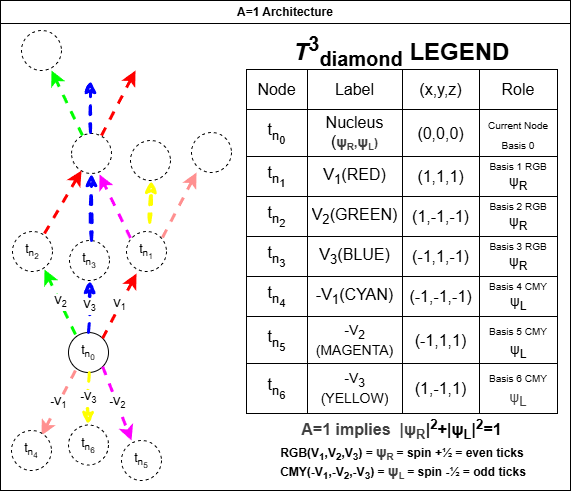
\includegraphics[width=\textwidth]{../figures/lattice_drawio.png}
\caption{The $\Tdiamond$ lattice architecture. The nucleus
node $t_{n_0}$ carries both Dirac spinor components $(\psi_R, \psi_L)$. 
RGB basis vectors constitute the right-handed sublattice ($\psi_R$, 
spin $+1/2$, even ticks) and CMY basis vectors the left-handed 
sublattice ($\psi_L$, spin $-1/2$, odd ticks). The A=1 constraint 
requires $|\psi_R|^2 + |\psi_L|^2 = 1$.}